%translator Savrov, date 27.04.13

\setcounter{Chapter}{5}

\Addition
{Tables}
{Tables}
{Tables}

\small \noindent\so{Table} V.1. Physical constants 
\fontsize{8.5pt}{7.5pt}\selectfont
\begin{center}
\begin{tabular}{p{5.3cm}p{5.5cm}}
%\hline
Speed of light in vacuum&
$c=2{.}997928\cdot10^{10}$ \cm/\s
\vspace{2pt}\\
Planck constant&
$h=6{.}6254\cdot10^{-27}\,\erg\cdot \s=$
\\&\hfill $=6{.}6254\cdot10^{-34}\,\Dj\cdot \s;$
\vspace{2pt}\\
&$\hbar=h/2\pi=1{.}0545\cdot10^{-27}\,\erg\cdot \s$
\vspace{2pt}\\
Boltzmann constant&
$k=1{.}38049\cdot10^{-16}\,\erg/\kelvin=$\\&\hfill$=1{.}38049\cdot10^{-23}\,\Dj/\kelvin$
\vspace{2pt}\\
Avogadro constant&
$N=6{.}0247\cdot10^{23}\,\mol^{-1}$
\vspace{2pt}\\
Stefan-Boltzmann constant&
$\sigma=5{.}6696\cdot10^{-5}\,\erg\cdot \cm^{-2}\cdot \kelvin^{-4}\cdot \s^{-1}=$
\\&\hfill$=5{.}6696\cdot10^{-8}\,\Vt\cdot \m^{-2}\cdot \kelvin^{-4}$
\vspace{2pt}\\
Wien' displacement law constant&
$\lambda_\textrm{max}\cdot T=0{.}297\,\cm\cdot \kelvin$
\vspace{2pt}\\
Energy\;corresponding to\;1\,eV (electron-volt)&
$1{.}6020\cdot10^{-12}\,\erg\Simeq1{.}6\cdot10^{-19}\,\Dj$
\vspace{2pt}\\
Rydberg constant for infinite mass&
$R_\infty=109737{.}31\,\cm^{-1}$
\vspace{2pt}\\
<<Radius of the first Bohr' orbit>> of hydrogen atom&
$a_0=5{.}29173\cdot10^{-9}\,\cm$
\vspace{2pt}\\
Atomic mass unit \aem.&
$931{.}16\,\MeV$
\vspace{2pt}\\
Electron Compton wavelength&
$\Lambda=2{.}4265\cdot10^{-10}\,\cm$
\vspace{2pt}\\
Bohr magneton&
$\mu_\textrm{B}=0{.}92733\cdot10^{-10}\,\erg\cdot \Gs^{-1}$
\vspace{2pt}\\
Nuclear magneton&
$\mu_\textrm{N}=0{.}50504\cdot10^{-23}\,\erg\cdot \Gs^{-1}$
\vspace{2pt}\\
Fine-structure constant&
$\alpha=7{.}2976\cdot10^{-3};\ 1/\alpha=137{.}03$
\vspace{2pt}\\
Electron mass&
$m_e=9{.}1086\cdot10^{-28}\,\g$
\vspace{2pt}\\
Electron charge&
$e=4{.}80294\cdot10^{-10}\:\textrm{esu}\Simeq$
\\&\hfill$\Simeq1{.}601\cdot10^{-19}\,\Kl$
\vspace{2pt}\\
Proton mass&
$m_p=1{.}67245\cdot10^{-24}\,\g=$\\&\hfill$=1{.}008142\,\aem.=938{.}72\,\MeV$
\vspace{2pt}\\
Magnetic moment of proton&
$\mu_p=+2{.}79275\,\mu_\textrm{�}$
\vspace{2pt}\\
Neutron mass&
$m_n=1{.}67476\cdot10^{-24}\,\g=$\\&\hfill$=1{.}008982\,\aem.=939{.}50\,\MeV$
\vspace{2pt}\\
Magnetic moment of neutron&
$\mu_n=-1{.}9128\,\mu_\textrm{�}$
\vspace{2pt}\\
$\alpha$-particle mass&
$m_\alpha=6{.}6442\cdot10^{-24}\,\g$
\vspace{2pt}\\
$\pi^\pm$-meson mass&
$m_{\pi^\pm}=273{.}4\,m_e$
\vspace{2pt}\\
Mean\:lifetime\:of\:$\pi^+$-\:and \mbox{$\pi^-$-mesons}&
$\tau_{\pi^+}=\tau_{\pi^-}=2{.}55\cdot10^{-8}\,\s$
\vspace{2pt}\\
$\pi^0$-meson mass&
$m_{\pi^0}=263{.}7\,m_e$
\vspace{2pt}\\
Mean lifetime of $\pi^0$-meson&
$\tau_{\pi^0}=1{.}05\cdot10^{-16}\,\s$
\vspace{2pt}\\
$\mu$-meson mass&
$m_\mu=207\,m_e$
\vspace{2pt}\\
Mean lifetime of muon&
$\tau_\mu=2{.}21\cdot10^{-6}\,\s$\\
%\hline
\end{tabular}
\end{center}


\newpage
{\small
\noindent\so{Table} V.2. Bright line wavelengths in spectra of neon and mercury 
\fontsize{8pt}{6pt}\selectfont
\begin{center}
{\begin{tabular}{l|c|c|l|c|c}
\hline
\multicolumn{3}{c|}{Neon} & \multicolumn{3}{c}{Mercury} \\ \hline
Color & Relative  & $\lambda$\,,\AA &
Color  & Relative  & $\lambda$\,,\AA \\
of line    & brightness        &                 &
of line    & brightness        &                  \\
         & (visual    &                 &
         & (visual    &                  \\
         & estimate)        &                 &
         & estimate)        &                  \\
\hline
Vermilion         &  10  &  6402 & Violet &  2  &    4046.56 \\
Red-orange     &  10  &  6143 & &  ---  &  4347.50 \\
Orange            &   5  &  5945 & Blue       &  8  &  4358.343 \\
Yellow               &  20  &  5853 &   &  ---  &  4398.62 \\
Light green       &   4  &  5765 &   &  ---  &   4487.48 \\
Green              &   6  &  5400 &    &  ---  &   4825.62 \\
Green              &   8  &  5330 &   Green     &  10 &   5460.742 \\
Green              &   5  &  5031 &    Yellow      &   8 &   5769.598 \\
Bluish-green         &   8  &  4849 &   Yellow      &  10 &   5790.659 \\
                     &      &       &   &  ---  &   6100.36 \\
                     &      &       &   &  ---  &  7301.68 \\
\hline
\end{tabular}}
\end{center}

%\vspace{8pt}
\small\noindent\so{Table} V.3. Free path of $\alpha$-particle in various materials
\fontsize{8pt}{6pt}\selectfont
\begin{center}
{\begin{tabular}{l|c|p{2cm}|c|c|c}\hline
$E, MeV $ \hspace{0.8pt}&\hspace{0.8pt} Al, $\mu$m \hspace{0.8pt}&\hspace{0.8pt} {Living tissue, $\vphantom{x^2}$ $\mu$m }\hspace{0.8pt}&\hspace{0.8pt} Water, $\mu$m \hspace{0.8pt}&\hspace{0.8pt} Air, cm \hspace{0.8pt}&\hspace{0.8pt} Lead, $\mu$m\\
\hline
\fontsize{8pt}{6pt}\selectfont
0.1    & 0.950 & \multicolumn{1}{c|}{1.03}  & 1.00 & 0.113 & 0.845 \\
0.5    & 2.56  & \multicolumn{1}{c|}{2.94}   & 2.87 & 0.309 & 2.23 \\
1.0    & 4.05  & \multicolumn{1}{c|}{5.06} & 4.96 & 0.499  & 3.78 \\
1.5    & 5.63  & \multicolumn{1}{c|}{7.50}  & 7.38 &  0.714 & 4.41 \\
2.0    & 7.38  & \multicolumn{1}{c|}{10.4}  & 10.2 & 0.966 & 5.61 \\
2.5    & 9.32  & \multicolumn{1}{c|}{13.6}  & 13.4 & 1.25  & 6.94 \\
3.0    & 11.5  & \multicolumn{1}{c|}{17.4}  & 17.1 & 1.58  & 8.39 \\
3.5    & 13.9  & \multicolumn{1}{c|}{21.6}  & 21.3 & 1.96  & 9.98 \\
4.0    & 16.5  & \multicolumn{1}{c|}{26.2}  & 25.8 & 2.37  & 11.7 \\
4.5    & 19.2  & \multicolumn{1}{c|}{31.2}  & 30.8 & 2.82  & 13.4 \\
5.0    & 22.2  & \multicolumn{1}{c|}{36.7}  & 36.2 & 3.29  & 15.3 \\
5.5    & 25.4  & \multicolumn{1}{c|}{42.6}  & 42.0 & 3.82  & 17.3 \\
6.0    & 28.8  & \multicolumn{1}{c|}{48.8}  & 48.2 & 4.37  & 19.4 \\
7.0    & 36.2  & \multicolumn{1}{c|}{62.4}  & 61.7 & 5.58  & 23.8 \\
8.0    &43.4   & \multicolumn{1}{c|}{78.0}  & 76.8 & 7.19  & 31.5 \\
9.0    & 52.2  & \multicolumn{1}{c|}{94.4}  & 93.0 & 8.66  & 36.0 \\
10.0   & 61.6  & \multicolumn{1}{c|}{112}   & 111  & 10.2  & 42.7 \\
\hline
\end{tabular}}
\end{center}
}

\noindent\small\so{Table} V.4. Attenuation coefficient of $\gamma$-rays in various materials (in cm$^{-1}$)
\fontsize{8pt}{6pt}\selectfont
\begin{center}
{\begin{tabular}{c|c|c|c|c|c|c|c}
\hline
$\hspace{6.5pt} E_\gamma$, MeV \hspace{6.5pt}& \hspace{6.5pt}Al\hspace{6.5pt} & \hspace{6.5pt}Cu\hspace{6.5pt}  &  \hspace{6.5pt}Fe\hspace{6.5pt}  &   \hspace{6.5pt}Pb\hspace{6.5pt}  &  \hspace{6.5pt}Water\hspace{6.5pt} & \hspace{6.5pt}Concrete\hspace{6.5pt} & \hspace{6.5pt}NaI\hspace{6.5pt} \\ \hline
0.1  & 0.456 & 4.117 & 2.928 & 62.03 & 0.171  & 0.397 & 6.055 \\
0.2  & 0.329 & 1.409 & 1.149 & 10.68 & 0.137  & 0.291 & 1.196 \\
0.3  & 0.281 & 1.000 & 0.787 & 4.275 & 0.119  & 0.251 & 0.602 \\
0.4  & 0.250 & 0.839 & 0.740 & 2.495 & 0.106  & 0.224 & 0.428 \\
0.5  & 0.228 & 0.745 & 0.661 & 1.724 & 0.0966 & 0.204 & 0.343 \\
0.6  & 0.210 & 0.679 & 0.605 & 1.349 & 0.0896 & 0.189 & 0.298 \\
0.8  & 0.184 & 0.588 & 0.526 & 0.982 & 0.0786 & 0.166 & 0.246 \\
1.0  & 0.166 & 0.526 & 0.471 & 0.798 & 0.0706 & 0.149 & 0.214 \\
1.5  & 0.135 & 0.430 & 0.382 & 0.581 & 0.0575 & 0.121 & 0.172 \\
2.0  & 0.117 & 0.377 & 0.337 & 0.518 & 0.0493 &  0.105 & 0.152 \\
5.0  & 0.076 & 0.285 & 0.246 & 0.483 & 0.0301 &  0.067 & 0.127 \\
\hline \end{tabular}} \end{center}


\noindent\small\so{Table} V.5. Reflectivity $\epsilon_{_T}$ of various materials (normal to the surface)
\fontsize{8.5pt}{7.5pt}\selectfont
\begin{center}
{\begin{tabular}{p{6cm}|c|c}
\hline
Material & Temperature, $^\circ$C & $\epsilon_{_T}$ \\ \hline
\qquad\qquad {\bf Metal } && \\
Aluminum polished & 50$\ldots$500 & 0.04$\ldots$0.06 \\
Aluminum coarse & 20$\ldots$50 & 0.06$\ldots$0.07 \\
Tungsten & 230 & 0.053 \\
Tungsten & 600$\ldots$1000 & 0.10$\ldots$0.16 \\
Tungsten & 1500$\ldots$2230 & 0.31 \\
Tungsten wire & 3300 & 0.39 \\
Cast iron coarse & 925$\ldots$1115 & 0.87$\ldots$0.95 \\
Gold polished & 225$\ldots$635 & 0.018$\ldots$0.035 \\
Gold polished & 100 & 0.02 \\
Copper polished & 50$\ldots$100 & 0.02 \\
Copper oxidized & 50 & 0.6$\ldots$0.7 \\
Molybdenum wire & 725$\ldots$2600 & 0.096$\ldots$0.292 \\
Nickel wire & 185$\ldots$1000 & 0.096$\ldots$0.186 \\
Nichrome wire pure  & 500$\ldots$1000 & 0.71$\ldots$0.79 \\
Platinum & 925$\ldots$1115 & 0.12$\ldots$0.17 \\
Crude iron melted & 1300$\ldots$1400 & 0.29$\ldots$0.29 \\
\qquad\qquad {\bf Various materials} && \\
Asbestos sheet & 40$\ldots$370 & 0.93$\ldots$0.95 \\
Concrete & 20 & 0.92 \\
White paper & 20 & 0.96 \\
Water layer (more than 0.1\,mm thick) & 0$\ldots$100 & 0.95$\ldots$0.96 \\
Calcium-silicate brick & 1230 & 0.66 \\
Human skin & 36 & 0.98 \\ \hline
\end{tabular}}
\end{center}

\vspace{8pt}
\small
%\renewcommand{\arraystretch}{0}
%\doublerulesep=6pt
\noindent\so{Table} V.6. Main properties of conductors

\vspace{6pt}
\noindent\includegraphics[width=11.3cm,height=6.5cm]{pic/Tabl_P6!.eps}

\newpage
\vspace*{-1cm}
\thispagestyle{empty}
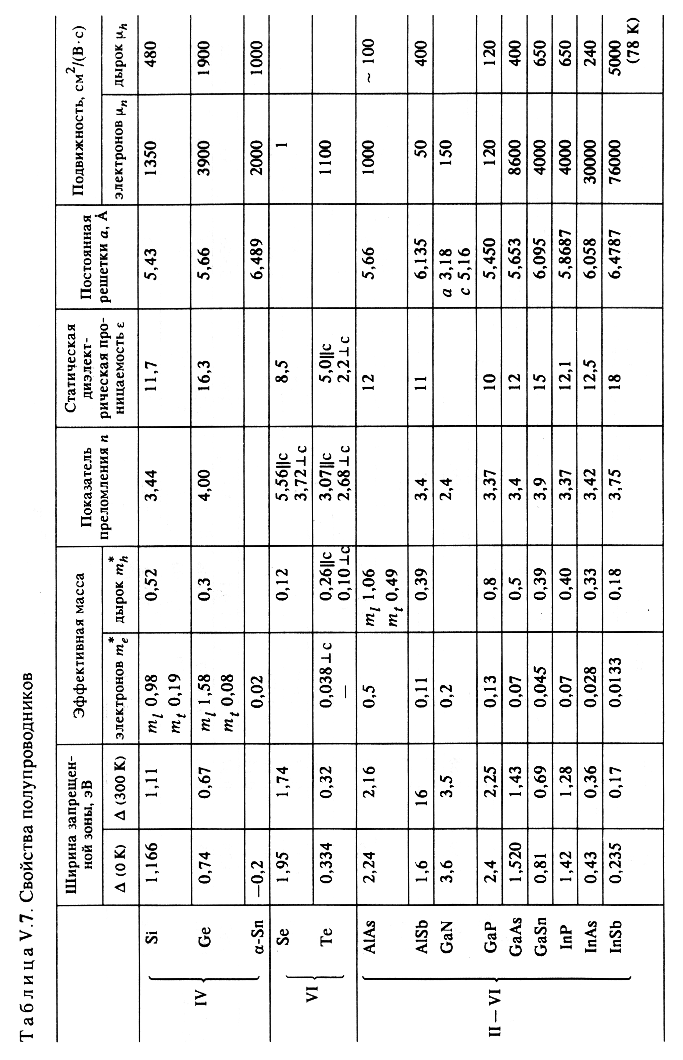
\includegraphics[width=11cm,height=17.4cm]{pic/TableV-8-1.eps}

\newpage
\vspace*{-1cm}
\thispagestyle{empty}
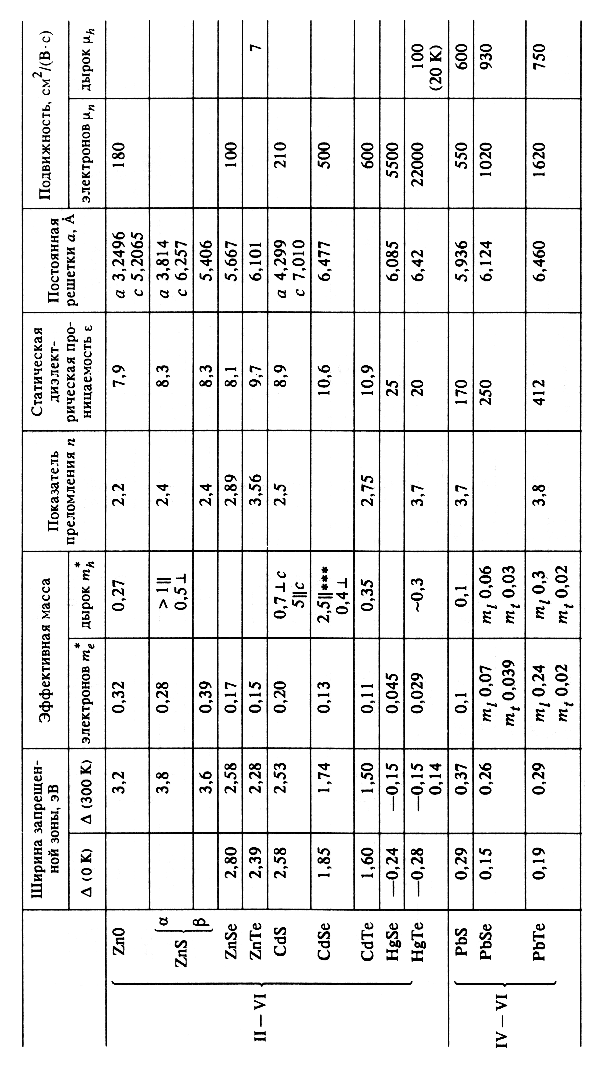
\includegraphics[width=9.6cm,height=17.4cm]{pic/TableV-8-2.eps}

\newpage
\small
\noindent\so{Table} V.8. Properties of magnetics

\vspace{6pt}
\noindent\includegraphics[width=11.3cm,height=9.4cm]{pic/Tabl_P7!.eps}

\vspace{18pt}
{\small
\noindent\so{Table} V.9. Critical temperature, Debye temperature, and critical magnetic field of some elements at zero temperature \fontsize{8pt}{8pt}\selectfont
\begin{center}
{\begin{tabular}{p{1.5cm}|c|c|c|c|p{1.5cm}|c|c|c}
\hline
Element & $T_\textrm{c},$K & $\Theta_\textrm{D}$\,,� & $H_\textrm{c},\,$Oe &\,&
Element & $T_\textrm{c},$K & $\Theta_\textrm{D}$\,,� & $H_\textrm{c},\,$Oe  \\
\hline
Al  &  1.19  &  420  & 105  &&   Pb  & 7.2    & 96    &  803      \\
Be  & 0.026  & 1160  &      &&   Sn  & 3.72   & 195   &  308      \\
Cd  & 0.55   & 300   & 29.6  &&  Ta  & 4.46   & 260   &  831        \\
Ga  & 1.09   & 317   & 58.9  &&  Ti  & 0.42   & 426   & 56         \\
Hg  & 4.15   & 90    & 390   &&  Tl  & 2.39   & 88    & 179       \\
In  & 3.4    & 109   & 289   &&  V   & 5.46   & 340   & 1167      \\
La  & 4.88   & 140   & 808   &&  W   & 0.015  & 390   & 1.07      \\
Mo  & 0.92   & 460   & 98    &&  Zn  & 0.85   & 310   & 52.5     \\
Nb  & 9.3    & 240   & 1980  &&  Zr  & 0.55   & 290   & 47.7      \\
\hline
\end{tabular}
\bigskip}
\end{center}

\newpage
\small
\so{Table} V.10. Parameters of HTS 
\begin{center}
\fontsize{8pt}{8pt}\selectfont
{\begin{tabular}{l|c|c|c|c|c|c}
\hline
Chemical compound &  $T_\textrm{c}\,$K & Number of  & $\lambda_{a,b}$, &
$\lambda_\textrm{c},$ &  $\xi_{a,b},$ & $\xi_\textrm{c}\,$, \\
          &    & CuO-layers & nm  & nm & nm  & nm  \\
\hline
La$_{1.85}$Sr$_{0.15}$CuO$_4$ & 40 & 1 & 80 & 430 & 3.7 & 0.7 \\
YBa$_2$Cu$_3$O$_7$            & 95 & 2 & 27 & 180 & 3.1 & 0.4 \\
Bi$_2$Sr$_2$CaCu$_2$O$_8$     & 95 & 2 & 25 & 500 & 3.8-1.8 & 0.2 \\
Bi$_2$Sr$_2$Ca$_2$Cu$_3$O$_{10}$ & 115 & 3& $<25$ & $>500$ &3 & $<0.2$\\
\hline
\end{tabular}}
\bigskip
\end{center}
}
\vspace{1cm}

\newpage
\thispagestyle{empty}
\vspace*{-1cm}
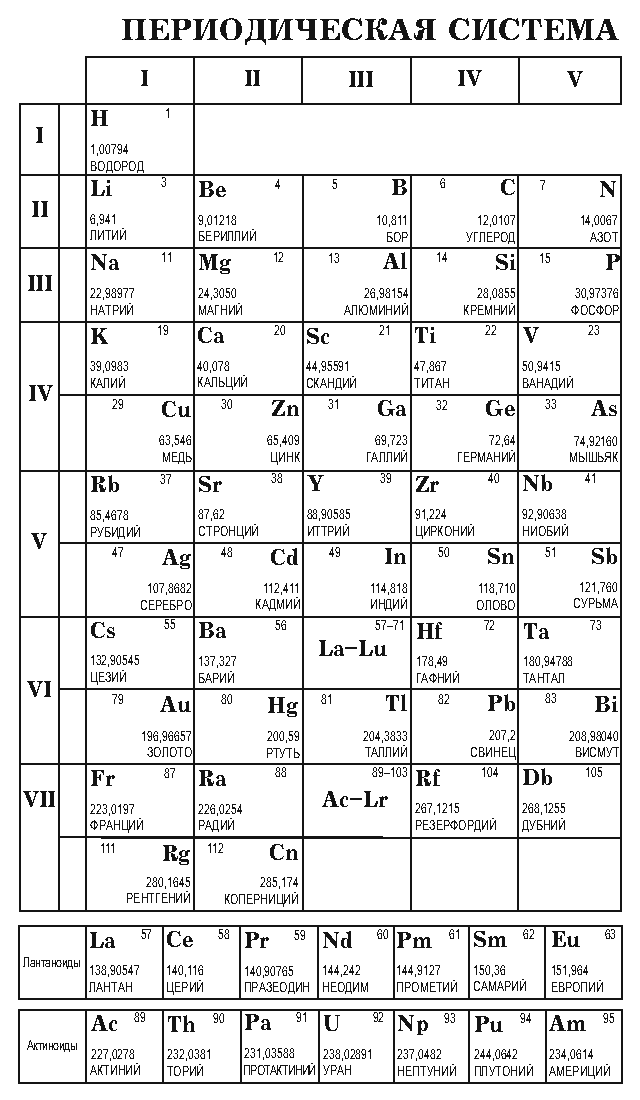
\includegraphics[width=10.22cm,height=18.03cm]{PIC/mend01.eps}

\newpage
\thispagestyle{empty}
\vspace*{-1cm}
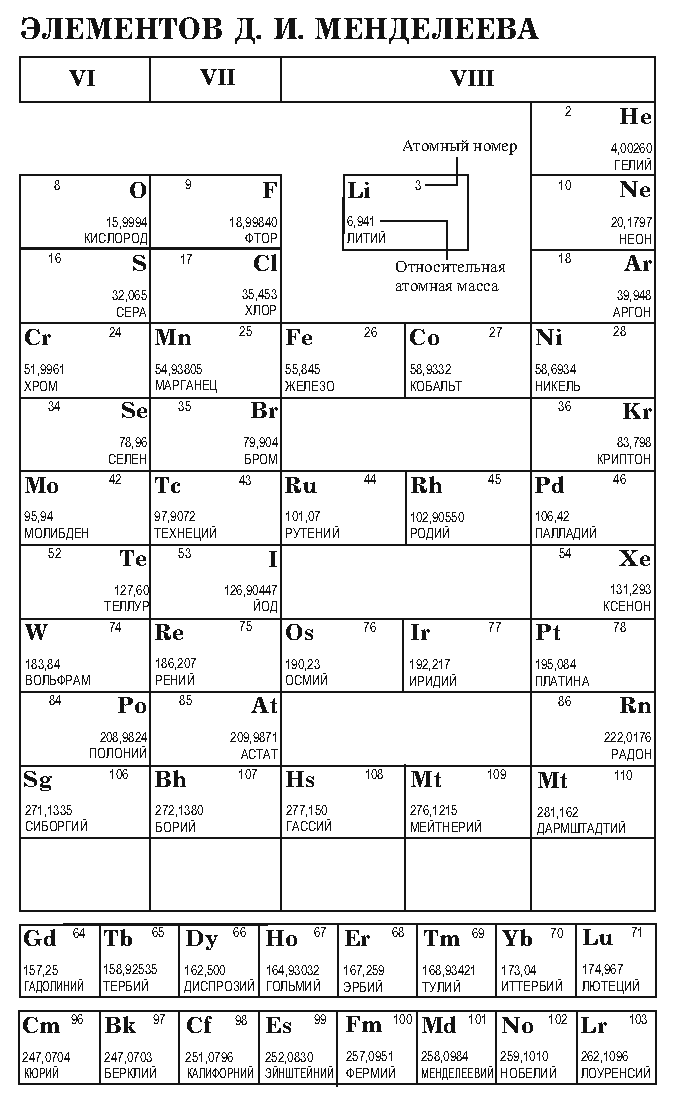
\includegraphics[width=10.78cm,height=18.09cm]{PIC/mend02.eps}

